% Auto-generated by 04_additional_analysis.R — do not edit
% y > 0: Underreacts  |  y < 0: Overreacts
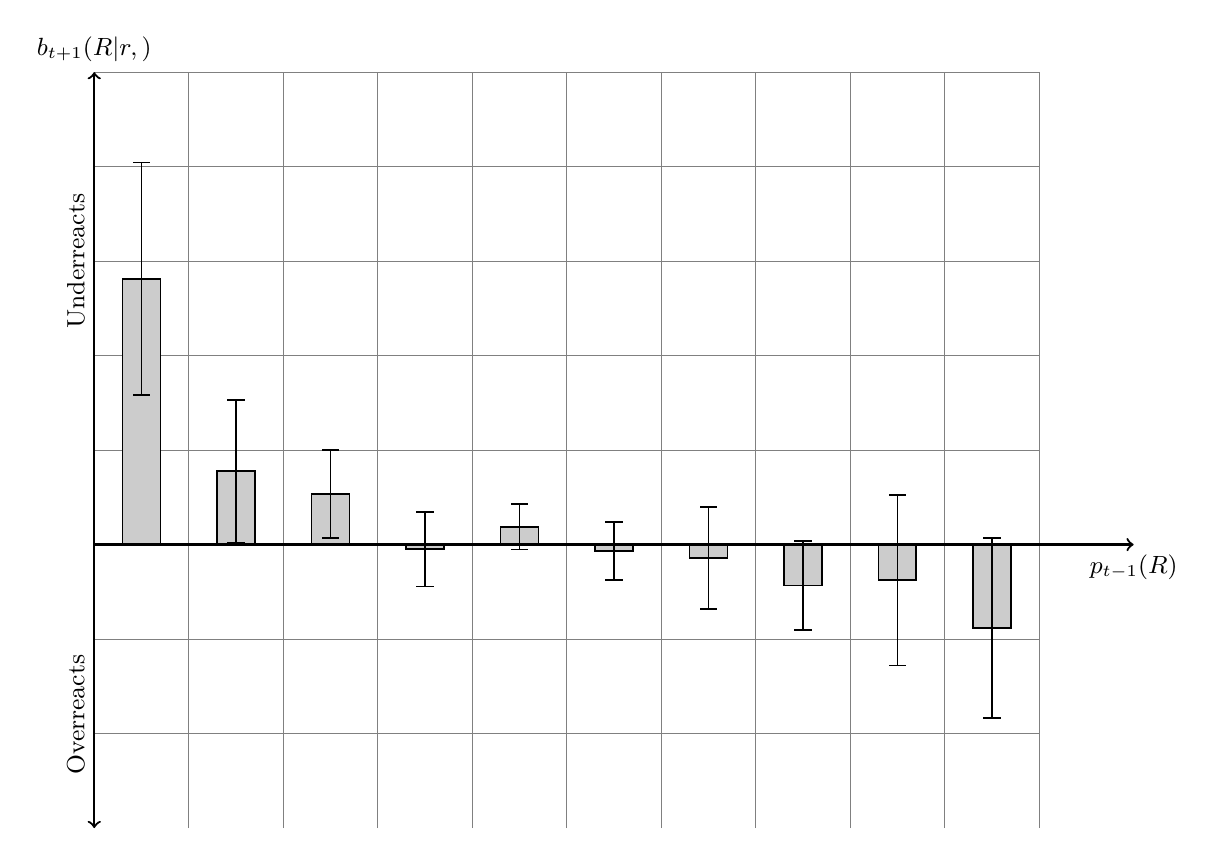
\begin{tikzpicture}[scale=12]
\draw[help lines,step=0.1] (0,-0.3) grid (1,0.5);
\filldraw[opaque,white!80!black] (0.03,0) rectangle (0.07,0.2812);
\draw[line width=0.6] (0.03,0) rectangle (0.07,0.2812);
\draw[line width=0.6,|-|] (0.05,0.1572) -- (0.05,0.4051);
\filldraw[opaque,white!80!black] (0.13,0) rectangle (0.17,0.0777);
\draw[line width=0.6] (0.13,0) rectangle (0.17,0.0777);
\draw[line width=0.6,|-|] (0.15,0.0014) -- (0.15,0.1540);
\filldraw[opaque,white!80!black] (0.23,0) rectangle (0.27,0.0532);
\draw[line width=0.6] (0.23,0) rectangle (0.27,0.0532);
\draw[line width=0.6,|-|] (0.25,0.0058) -- (0.25,0.1007);
\filldraw[opaque,white!80!black] (0.33,0) rectangle (0.37,-0.0049);
\draw[line width=0.6] (0.33,0) rectangle (0.37,-0.0049);
\draw[line width=0.6,|-|] (0.35,-0.0453) -- (0.35,0.0355);
\filldraw[opaque,white!80!black] (0.43,0) rectangle (0.47,0.0188);
\draw[line width=0.6] (0.43,0) rectangle (0.47,0.0188);
\draw[line width=0.6,|-|] (0.45,-0.0061) -- (0.45,0.0437);
\filldraw[opaque,white!80!black] (0.53,0) rectangle (0.57,-0.0067);
\draw[line width=0.6] (0.53,0) rectangle (0.57,-0.0067);
\draw[line width=0.6,|-|] (0.55,-0.0383) -- (0.55,0.0248);
\filldraw[opaque,white!80!black] (0.63,0) rectangle (0.67,-0.0142);
\draw[line width=0.6] (0.63,0) rectangle (0.67,-0.0142);
\draw[line width=0.6,|-|] (0.65,-0.0692) -- (0.65,0.0409);
\filldraw[opaque,white!80!black] (0.73,0) rectangle (0.77,-0.0432);
\draw[line width=0.6] (0.73,0) rectangle (0.77,-0.0432);
\draw[line width=0.6,|-|] (0.75,-0.0915) -- (0.75,0.0050);
\filldraw[opaque,white!80!black] (0.83,0) rectangle (0.87,-0.0376);
\draw[line width=0.6] (0.83,0) rectangle (0.87,-0.0376);
\draw[line width=0.6,|-|] (0.85,-0.1289) -- (0.85,0.0536);
\filldraw[opaque,white!80!black] (0.93,0) rectangle (0.97,-0.0883);
\draw[line width=0.6] (0.93,0) rectangle (0.97,-0.0883);
\draw[line width=0.6,|-|] (0.95,-0.1842) -- (0.95,0.0077);
\draw[line width=0.8,->]  (0,0) -- (1.1,0) node[below] {\small{$p_{t-1}(R)$}};
\draw[line width=0.8,<->] (0,-0.3) -- (0,0.5) node[above] {\small{$b_{t+1}(R|r,\xmark)$}};
\draw (0,0.30) node[above,rotate=90] {\small{Underreacts}};
\draw (0,-0.18) node[above,rotate=90] {\small{Overreacts}};
% ADD THEORY CURVE BELOW
\end{tikzpicture}
